\documentclass[a4paper,11pt]{article}

\usepackage[T1]{fontenc}
\usepackage[french]{babel}
\usepackage[utf8x]{inputenc}
%\usepackage{palatino} %change la police d'écriture.
\usepackage{lipsum} %pour avoir un texte, en latin, déja écrit, inutile dans 99,999999 % du temps.


%modules mathématiques :
\usepackage{amsmath}
\usepackage{amssymb}
\usepackage{mathrsfs} %pour avoir un police d'écriture anglo-saxonne en mode mathématique.
\usepackage{amsthm}
\usepackage{amssymb} %symboles en plus.
\usepackage{amsfonts}
\usepackage{a4wide}
%autres packages :
\usepackage{verbatim} %pour pouvoir changer de police dans le document.
\usepackage{mathptmx} %pour utiliser une autre police
\usepackage{dsfont}
\usepackage{graphicx} %pour pouvoir faire des graphes.
\usepackage{color} %pour mettre de la couleur
\definecolor{bblack}{cmyk}{0,0,0,1} 
\usepackage[colorlinks=true,linkcolor = black,urlcolor=black]{hyperref} %pour les liens hypertextes
\usepackage{float}
% \usepackage{Sweave} %pour du code R
% \usepackage{mhchem}
%si on veut mettre du code python
\usepackage{listings}
\definecolor{dkgreen}{rgb}{0,0.4,0}
\definecolor{gray}{rgb}{0.5,0.5,0.5}
\definecolor{mauve}{rgb}{0.58,0,0.82}
\definecolor{dkyellow}{cmyk}{0, 0, 0.2, 0}
\lstset{
  language=Python,                % the language of the code
  basicstyle= \footnotesize,      % the size of the fonts that are used for the code
  numbers=left,                   % where to put the line-numbers
  numberstyle=\tiny\color{gray},  % the style that is used for the line-numbers
  stepnumber=2,                   % the step between two line-numbers. If it's 1, each line 
                                  % will be numbered
  showspaces=false,               % show spaces adding particular underscores
  showtabs=false,                 % show tabs within strings adding particular underscores
  frame=single,                   % adds a frame around the code
  rulecolor=\color{black},        % if not set, the frame-color may be changed on line-breaks within not-black text (e.g. commens (green here))
  tabsize=2,                      % sets default tabsize to 2 spaces
  captionpos=b,                   % sets the caption-position to bottom
  breaklines=true,                % sets automatic line breaking
  breakatwhitespace=false,        % sets if automatic breaks should only happen at whitespace
  keywordstyle=\color{blue},      % keyword style
  commentstyle=\color{dkgreen},   % comment style
  stringstyle=\color{mauve},       % string literal style
  backgroundcolor=\color{dkyellow},      % choose the background color. You must add \usepackage{color}
}
%%%%%%%%%%%%%%%%%%%%%%%%%%%

%%%%%% Pour reduire les marges ! %%%%%%%%%%%%%%%
%\setlength{\textwidth}{15cm} %Largeur du texte : n
%\setlength{\marginparwidth}{0cm}
%\setlength{\oddsidemargin}{0.5cm} %m avec 2m+n = 16 pour que ca marche bien.
%\setlength{\headheight}{0cm}
%\setlength{\topmargin}{2cm} %hauteur marge d'en haut
%\setlength{\headsep}{0cm} %hauteur de l'en tete
%\setlength{\textheight}{21cm} %hauteur du texte
%\setlength{\footskip}{0cm} %hauteur du pied de page
%\setlength{\marginparsep}{0cm}
%%%%%% Commandes pour structurer le texte %%%%%%%
%\part
%\section
%\subsection
%\subsubsection

%Pour énumérer, dans une section ou une sous-section :
%\begin{enumerate}
%\item texte
%\item texte2 etc.
%\end{enumerate}

%\vspace{n pt} : met un espace de n point(s) entre les paragraphes. Attention à l'utilisation.
%\vspace{6 ex} : met un espace de 6 hauteurs de police entre les paragraphes. Attention à l'utilisation.
%\vspace*{...} : force l'espace, même si c'est au début ou à la fin d'une page. Tres attention a l'utilisation.

% \\ pour passer une ligne
% \newpage pour écrire ce qui suit sur une nouvelle page
% \clearpage : pour ne rien ecrire de plus sur la page en cours

%%%%%%%%%%%%%%%%%%%%%%%%%%%%%%%%%%%%%%%%%%%%%%%%%%

%%%%%%%%%%%%% Deux modes maths %%%%%%%%%%%%%%%%%%%
% mettre entre $, ex : $ 2+2 = 4$ 
% mettre entre \[ \], ex : \[ 2+2 = 4 \].
%Attention, rendus différents
%%%%%%%%%%%%%%%%%%%%%%%%%%%%%%%%%%%%%%%%%%%%%%%%%%

%%%%%%%%%%%%Pour faire un calcul, centré sur les = %%%%%%%%%%%%%%%
%\begin{align*}
%calcul, tout sera déja en mode maths.
%a &= b
%&= c+d-E etc.
%\end{align*}
%%%%%%%%%%%%%%%%%%%%%%%%%%%%%%%%%%%%%%%%%%%%%%%%%%



%%%%%%%%%%%% Pour mettre en valeur un résultat %%%%%%%%%%%%%%%%%%%
%\begin{abstract}
 %résultat\begin{abstract}
%\end{abstract}
% Attention au rendu, il faudrait réussir à enlever la phrase en gras juste au dessus.
%%%%%%%%%%%%%%%%%%%%%%%%%%%%%%%%%%%%%%%%%%%%%%%%%%%%%%%%%%%%%%%%%%%

%%%%%%%%%%%% Pour des références %%%%%%%%%%%%%%%%%%%%
%\label{ref1}
%\ref{ref1}
%\pageref{ref1}
%%%%%%%%%%%%%%%%%%%%%%%%%%%%%%%%%%%%%%%%%%%%%%%%%%%%%

%%%%%%%%%%%% Pour des fleches stylees %%%%%%%%%%%%%%%
%\xrightarrow[nce qu'il y aura en dessous]{ce qu'il y aura au dessus}
%ex :\xrightarrow[n \to \infty]{P-ps}
%%%%%%%%%%%%%%%%%%%%%%%%%%%%%%%%%%%%%%%%%%%%%%%%%%%%%


%%%%%%%%%%% Pour rajouter des trucs en dessous (au dessus d'une expression) %%%%%%%%%%%%%%%%%%
%\underset{ce qu'il y a en dessous}{ce qu'il y a au dessus}
%\underset{n\to \infty}{=}

%\overset{ce qu'il y a au dessus}{ce qu'il y a en dessous}
%\overset{n\to \infty}{=}
%%%%%%%%%%%%%%%%%%%%%%%%%%%%%%%%%%%%%%%%%%%%%%%%%%%%%%

%%%%%%%%%%% Pour inclure un graphique %%%%%%%%%%%%%%%%
%\includegraphics[hauteur]{nom de l'image} % L'image doit être dans le même fichier que le fichier.tex.
%ex : \includegraphics[width=11cm]{unif_n10.jpeg}
%%%%%%%%%%%%%%%%%%%%%%%%%%%%%%%%%%%%%%%%%%%%%%%%%%%%%%
                    
                     
% mathbb pour les corps R, C ...
% mathcal pour les lettres caligraphiques (tribus etc.)
% mathfrak pour les lettres ghotiques
% mathbf pour les lettres en gras

%%%%%%%%%%%% Pour le titre la date et autres infos du pdf %%%%%%%%%%%%%
% \title{Book Report on : Heat Wave}
% \author{Benjamin Donnot}
% \date{}

%\pdfinfo{%
%  /Title    ()
%  /Author   ()
%  /Creator  ()
%  /Producer ()
 % /Subject  ()
%  /Keywords ()
%}
%%%%%%%%%%%%%%%%%%%%%%%%%%%%%%%%%%%%%%%%%%%%%%%%%%%%%%%%%%%%%%%%%%%%%%%%%%

%%%%%%%%%%%%%%%%%%%%%%% Affichage du titre ou autre %%%%%%%%%%%%%%%%%%%%%%
% \maketitle : affiche le titre
%%%% \tableofcontents : pour faire une table des matières
%%%%%%%%%%%%%%%%%%%%%%%%%%%%%%%%%%%%%%%%%%%%%%%%%%%%%%%%%%%%%%%%%%%%%%%%%%

%%%%%%%%%%%%Pour des entetes stylees%%%%%%%%%%%%%%%%%%%
\makeatletter
\def\clap#1{\hbox to 0pt{\hss #1\hss}}%
\def\ligne#1{%
\hbox to \hsize{%
\vbox{\centering #1}}}%
\def\haut#1#2#3{%
\hbox to \hsize{%
\rlap{\vtop{\raggedright #1}}%
\hss
\clap{\vtop{\centering #2}}%
\hss
\llap{\vtop{\raggedleft #3}}}}%
\def\bas#1#2#3{%
\hbox to \hsize{%
\rlap{\vbox{\raggedright #1}}%
\hss
\clap{\vbox{\centering #2}}%
\hss
\llap{\vbox{\raggedleft #3}}}}%
\def\maketitle{%
\thispagestyle{empty}\vbox to \vsize{%
\haut{}{\@blurb}{}
\vfill
\vspace{1cm}
\begin{flushleft}
\usefont{OT1}{ptm}{m}{n}
\huge \@title
\end{flushleft}
\par
\hrule height 4pt
\par
\begin{flushright}
\usefont{OT1}{phv}{m}{n}
\Large \@author
\par
\end{flushright}
\vspace{1cm}
\begin{center}
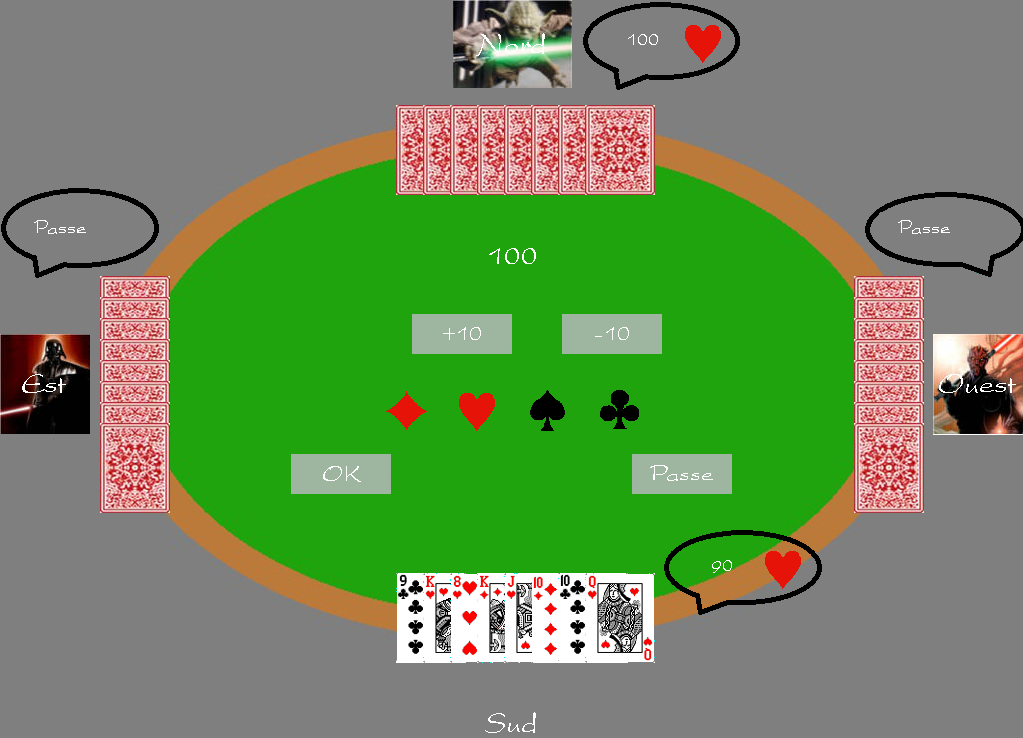
\includegraphics[width=13cm]{img/Coinche.png}
\end{center}

\vfill
\vfill
\bas{}{}{}
}
\cleardoublepage
}
\def\date#1{\def\@date{#1}}
\def\author#1{\def\@author{#1}}
\def\title#1{\def\@title{#1}}
\def\location#1{\def\@location{#1}}
\def\blurb#1{\def\@blurb{#1}}

\makeatother

\date{3 Mai 2015}
\title{Projet Informatique : Jeu de Coinche}
\author{Benjamin DONNOT}
\location{}
\blurb{}

\renewcommand{\thesection}{\Roman{section}}
\renewcommand{\thesubsection}{\Roman{section}.\arabic{subsection}}
\renewcommand{\thesubsubsection}{\Roman{section}.\arabic{subsection}.\roman{subsection}}
%%%%%%%%%Pour l'en-tete et le pied de page%%%%%%%%%%%%%%%%%%
\usepackage{fancyhdr}
\pagestyle{fancy}
\usepackage{lastpage}
\renewcommand\headrulewidth{1pt}
\renewcommand\footrulewidth{1pt}
\fancyfoot[C]{Projet informatique\\ \textbf{Page \thepage/\pageref{LastPage}}}
\fancyfoot[R]{ENSAE 3\ieme{} année \\ Data Science}
\fancyfoot[L]{Benjamin DONNOT }
\fancyhead[L]{}
\begin{document}
\maketitle
\tableofcontents
\clearpage
\section*{Introduction}
\addcontentsline{toc}{section}{Introduction} 
Depuis le cours de Python de première année, j'ai découvert un champ assez vaste de l'informatique : celui de l'\textit{intelligence artificielle} (IA). Ce terme, assez générique, a plusieurs sens. Ce que j'entends par "intelligence artificielle" dans tout ce rapport, et plus généralement dans le projet tout entier, c'est la capacité pour un ordinateur à prendre des décisions "cohérentes" et ainsi à jouer "convenablement" à la coinche. \\

La "Coinche", comme de nombreux jeux de cartes, ne se joue pas en "information parfaite" : les cartes des adversaires sont cachées ! Résoudre\footnote{Entendre ici : performer aussi bien que les humains en général.} un jeu de coinche pourrait donc permettre de faire des avancées dans certains types de problèmes rencontrés dans la vie de tous les jours o\`u nous sommes amenés à prendre des décisions dans un environnement incertain\footnote{Qui est nettement plus compliqué que l'environnement simplifié du jeu de Coinche.}. Ainsi, il n'est pas rare que la recherche en IA se concentre sur des jeux. C'était notamment le cas au début des années 90 avec IBM et "Deep Blue", le premier ordinateur a avoir battu un grand maître aux échecs\footnote{Cette victoire a suscité de nombreuses polémiques qui ne seront pas abordées ici, car ce n'est pas le sujet. Toujours est-il qu'aujourd'hui, il est communément admis que les ordinateurs jouent mieux que les humains aux échecs.}. Actuellement, de nombreuses compétitions de jeux voient affronter les meilleurs programmes informatiques du monde, notamment au Go\footnote{On pourra se reporter au "Computer Go" :  \url{http://en.wikipedia.org/wiki/Computer_Go}.}, ou encore le Bridge\footnote{Jeu relativement proche de la Coinche, mais beaucoup plus populaire outre Manche et outre Atlantique. On pourra se reporter au "Computer Bridge" : \url{http://en.wikipedia.org/wiki/Computer_bridge}.}. D'un point de vue fondamental, se concentrer sur des jeux présente plusieurs intérêts : les données sont faciles à acquérir (il suffit de faire jouer un ordinateur contre lui-même un grand nombre de fois pour avoir des parties simulées), et ils représentent souvent des versions (très) simplifiées de problèmes réels. \\

Ce type de jeu de cartes est également en relation avec le module \textit{statistique et apprentissage}, dans lequel j'effectue ma 3\ieme{} année à l'ENSAE. L'"Intelligence Artificielle" et le "Machine Learning" sont des champs très proches, notamment lorsque l'environnement n'est pas entièrement connu par les acteurs. Dans ce cas, il faut souvent faire des statistiques afin de prendre la meilleure décision possible. Il n'est donc pas surprenant que les meilleurs algorithmes de Bridge actuels reposent sur des techniques "Monte Carlo" : on va simuler un grand nombre de jeux possibles, tenter de résoudre chaque jeu en information complète, puis agréger tous ces résultats pour en tirer la meilleure action à faire dans l'environnement incertain de départ. On pourra se reporter à la partie \ref{sec:MCPlay} page \pageref{sec:MCPlay} ci après pour plus d'informations. \\
J'ai également tenu à coder un jeu de Coinche car c'est un jeu auquel j'aime jouer pendant mes loisirs en tant qu'amateur.

En 2\ieme{} année, j'ai pu suivre le cours de c++, et j'ai réalisé un projet de Belote\footnote{Les sources de l'époque sont disponibles dans le répertoire SVN suivant : \url{https://subversion.assembla.com/svn/belote_cpp/}.}. Pour la réalisation de ce projet, je disposais donc d'une interface graphique correcte\footnote{Celle-ci, même si je l'ai recodée en grande partie pendant ma césure, n'est pas exempte de défauts, mais ne fait pas l'objet de ce rapport, ni même de ce projet.}. C'est aussi parce que cette interface était convenable que j'ai porté mon dévolu sur ce jeu de Coinche. De cette façon j'ai pu me concentrer sur ce qui, pour moi, est l'essentiel : l'\textbf{\textit{IA}}. \\
Au cours de ma deuxième année, je m'étais concentré sur deux aspects principaux : l'interface graphique, ainsi que la prise. La partie "jeu" en elle-même n'avait été que peu étudiée, et faisait l'objet d'une implémentation rudimentaire. Ce projet aura donc pour but de réaliser une intelligence artificielle capable de jouer correctement sur toute une partie de Coinche, en utilisant des techniques Monte Carlo décrites précédemment. \\

Ce projet a été principalement codé grâce à codeblocks dans un environnement Linux (Ubuntu 14.04 LTS), le compilateur principal est gcc 4.8.2. \\
Ce projet dépend également de boost (pour la partie génération de nombres aléatoires : cette dépendance sera sûrement enlevée dans un futur proche) et utilise le standard c++11.\\
Parce que je voulais que mon jeu soit également disponible à des personnes utilisant windows, je l'ai également compilé avec codeblocks sous windows (avec le compilateur MingW). Comme ce compilateur ne me satisfaisait plus, j'ai essayé de faire en sorte que ce projet soit compilable avec visual studio (Visual C++). L'étape de compilation fonctionne, mais il reste quelques bugs dans l'application compilée. Je n'ai pas toujours eu le temps de m'y attardé, d'autant que ces bugs n'apparaissaient pas avec GCC...

Le fonctionnement est donc garanti avec :
\begin{itemize}
\item gcc 4.8.2
\item codeblocks 13.12
\item boost 1.55
\item SDL 1.2 (version de développement)
\end{itemize}

La compilation avec Visual Studio reste "expérimentale".
\clearpage
\section{Préambule}
\subsection{Architecture}
Ce code est relativement volumineux, il contient plus de $7~000$ lignes de codes\footnote{Sans compter les commentaires, ni les lignes avec un seul caractère, comme '$\{$' par exemple. Plus de $10~000$ sont présentes au total.}. Il compte 73 fichier de déclaration (.h) et 45 fichier source (.cpp) pour environ 90 définitions de classes. Le détail de chaque fichier, ou même de chaque classe est donc beaucoup trop long pour être présenté en exhaustivité dans ce rapport, et présenterait peu d'intérêt. \\
En revanche, chaque "header" est construit de la même façon. Tout d'abord, une courte description des classes qu'il contient est présentée, ensuite d'autres "headers" sont inclus, puis enfin des "TO DO" sont présents. Encore une fois, comme ce projet s'inscrit pour moi dans une vision à plus long terme que la validation de ce cours. Ces "TO DO" sont présents parce que beaucoup d'aspects restent à améliorer, et il est donc important pour moi de garder quelques parts les améliorations auxquelles je pense.\\
Cette partie sera uniquement dédiée à l'architecture du code en général. On pourra se reporter au header définissant une classe si l'utilité ou le fonctionnement de celle-ci n'est pas claire. \\

On rentre dans le programme via le fichier "\textit{main.cpp}". Celui-ci va déclarer une instance de la classe "\textit{Game\_Coinche}". Cette classe a pour but d'orchester le jeu. Elle ne va rien calculer, mais va faire en sorte que les différentes phases se déroulent sans accros les unes après les autres. Un point est a soulevé ici. Pour ce projet, je n'ai pas fait de tests unitaires et les erreurs ne sont pas gérées. Une première piste d'amélioration est donc clairement la gestion des exceptions, et la création de tests unitaires, notamment parce que le projet grossit. \\

Ce sont d'autres classes qui sont chargées de gérer quel joueur fait quelle action à quel moment. Il s'agit des classes "\textit{Cards\_Deck}" (qui va donner les cartes), "\textit{Bidding}" (qui va organiser la phase des enchères) et "\textit{Trick}" qui assure le bon déroulement des 8 plis. Globalement, ces classes vont donner des instructions à la classes "\textit{Player}" qui est chargée de faire les actions à proprement parler. \\

Pour l'instant, la classe "\textit{Player}" se divise en deux : "\textit{Player\_AI}" et "\textit{Player\_Human}" qui gère respectivement les joueurs "artificiels" (IA) et les joueurs humains. Dans l'architecture actuelle, la classe joueur va faire descendre les informations nécessaires à la prise de décision à des "wrappers" spécialisés ("\textit{AIPlayMonteCarlo}", "\textit{AIPlayScores}" ou "\textit{Player\_Bid\_Graphic}" par exemple). Dans la version précédente (projet Belote de 2A), les différentes façon de jouer étaient gérées via un polymorphisme dynamique (fonction "play" virtuelle) : ceci nécessitait de créer une classe par type de joueur IA et une pour les joueurs humains. Aujourd'hui, l'utilisation de "templates" et de \textit{wrappers} permettrait de s'en passer et de n'avoir qu'une seule classe "\textit{Player}" : ce serait au moment de la compilation (et non de l'exécution) que le choix du \textit{wrapper} serait "décidé". \\

\subsection{Limitations principales}

En plus des différents "TO DO" dans le code, le jeu est encore loin d'être parfait. Certaines limitations impactent directement le jeu et n'ont pas encore été implémentées. On peut notamment citer :
\begin{itemize}
\item Les variantes de jeu 'tout atout' et 'sans atout' n'ont pas été prises en compte. Ces variantes modifient profondément les règles du jeu\footnote{Avec la disparition de l'atout...}, et j'ai préféré me concentrer sur la façon de jouer plutôt que d'adapter le code historique (de 2A) de façon à ce qu'il puisse supporter ces variantes.
\item La belote (fait d'avoir la dame \textit{et} le roi dans la couleur d'atout) n'est également pas prise en compte. Il aurait fallu pour cela adapter l'interface graphique, je n'ai pas jugé cette tâche prioritaire.
\item La coinche est également absente. Lors de la phase des enchères, on peut "coincher" pour signifier à l'adversaire qu'il ne fera pas le contrat qu'il a annoncé. Ceci modifie entre autre les règles de comptage des points, et n'a pas été implémenté car j'ai laissé de côté la phase des enchères pour me concentrer sur le phase de jeu.
\item Pour les mêmes raisons, la prise a été mise de côté. Les joueurs IA prennent selon des critères très rudimentaires.
\item Il n'y a pas de prise en charge d'un "protocole réseau". On ne peut jouer que seul contre l'ordinateur. Deux joueurs humains ne peuvent pas jouer une même partie en même temps.
\end{itemize}

\subsection{Interface graphique}

Une des raisons qui m'ont poussées à choisir ce sujet était le fait que j'avais déjà codé une interface graphique pendant que j'étais en 2A.\\
La librairie utilisée est \textit{SDL 1.2}, une librairie codée en C. Durant ce projet, j'ai été plusieurs fois confronté à des problèmes d'utilisation, parce que les fonctions que j'avais codées n'étaient pas simple à utiliser et assez instable. Pour l'interface graphique,  j'avais eu recourt à une architecture particulière, basée sur l'héritage multiple, qui rend les classes que j'ai créées assez "obscures", même pour moi qui les ais codées. \\
Ce pourrait donc être une bonne idée de recoder cette partie. Mais, comme une nouvelle version de cette librairie est maintenant disponible (la version 2.0), je pourrai également en profiter pour mettre à jour mon code. Je pense à également à re-coder l'interface pour utiliser \textit{SFML} une autre librairie graphique qui a le mérite d'être codée en C++.\\
%Et, par la même occasion, pourquoi utiliser une librairie en C alors que le projet est codé en c++ ? Je pense donc changer de librairie pour l'interface graphique et utiliser SFML, qui a le mérite de ne pas utiliser de pointeurs, à ma connaissance. \\

Dans cette sous-partie, je voulais également mentionner que, par rapport à l'interface originale, j'ai ajouté une partie "Multi-Threading"\footnote{En utilisant les header de la librairie standard "thread" et "future". Ceci implique entre autre que le projet ne puisse plus être compilé avec Codeblocks sous windows (qui utilise MingW), parce que le compilateur en question ne prend pas en compte ces librairies.}. Lorsqu'un joueur IA prend une décision pour jouer une carte, l'interface graphique ne se fige pas, contrairement à ce qui se serait passer si l'application n'utilisait qu'un seul "thread".

\subsection{Débugage}

Une telle application a connu pas mal de bugs. Aujourd'hui, je pense en avoir éliminé une grande partie. Ceci n'a pas été facile, d'autant que les débugueurs ralentissent grandement la vitesse d'exécution des programmes, et que certains bugs apparaissaient au bout de plusieurs minutes d'exécution "standard"\footnote{Comprendre ici : sans que le debugueur ne soit activé.}. Pour arriver au même endroit avec un débugueur, il aurait sans doute fallu attendre plusieurs dizaines de minutes, ce qui est très frustrant. \\

J'ai donc beaucoup pratiqué le débugueur via l'affichage à l'écran. Pour que le code que j'ai créé soit relativement générique, j'ai donc codé deux wrappers, codés dans le fichier "\textit{DebugWithPrint}". Il s'agit de la classe "\textit{WrapperPrint}". Cette classe est templaté par un entier. En général elle ne fait rien, mais une spécialisation de cette classe a lieu lorsque cet entier vaut $1$ et dans ce cas elle va afficher (via "vfprintf") du texte dans la console. \\
Cette petite astuce m'a permis de localiser des bugs de façon assez rapide. Elle permet également de ne pas ralentir l'exécution du programme (cela prend du temps d'afficher beaucoup de texte) une fois que le bug a été trouvé, tout en ne déclarant que quelques variables.
\clearpage
\section{\textit{Intelligence Artificielle} : premier pas}
Les deux prochaines parties vont rentrer plus dans les détails de l'intelligence artificielle lors de la phase de jeu. Il serait sans doute plus facile de coder une intelligence artificielle qui est en information parfaite. Mais ceci ferait perdre beaucoup d'intérêt à ce projet. Donc, les 3 joueurs gérés par l'ordinateur ne connaissent pas le jeu des autres, et n'ont donc accès qu'au leur.\\

Cette partie va se concentrer sur l'architecture du code concernant l'IA, ainsi que sur les IA "basiques" qui sont aujourd'hui implémentées.
\subsection{Architecture}
Les décisions que l'ordinateur doit prendre concernant le jeu sont prises via la méthode "what\_card\_do\_i\_play". Dans cette méthode, il s'agit de choisir une parmi une liste de "cartes jouables"\footnote{Ces cartes sont déjà connues à ce stade.}. Aujourd'hui, pour le joueur IA, cette méthode se contente (dans le cas o\`u l'application n'est pas multi-threadée) de rediriger la sortie du wrapper "PlayAI" (template). \\

\`A ce jour, ce wrapper peut être de 3 natures différentes : 
\begin{itemize}
\item "\textit{AIPlayRandom}" : va permettre au joueur de jouer une carte aléatoire. On parlera dans ce cas d'\textbf{IA aléatoire}.
\item "\textit{AIPlayScores}" : va permettre au joueur de jouer une carte selon des scores prédéfinis. On parlera plus dans ce cas d'\textbf{IA scores}.
\item "\textit{AIPlayMonteCarlo}" : va jouer avec la méthode "Monte Carlo". On pourra se reporter à la partie \ref{sec:MCPlay} pour plus d'informations. On appellera ce type de jeu "\textbf{IA Monte Carlo}". \\
\end{itemize}

Cette architecture permet rapidement de créer de nouveaux types d'IA (avant, il aurait fallu recréer une classe héritant de "\textit{Player\_AI}"), mais permet également de faire interagir des types d'IA entre eux.\\
Par exemple, il y a deux sous-façons de jouer pour une "IA Mont Carlo" : la première est de simuler des parties o\`u les joueurs jouent aléatoirement (\textbf{IA Monte Carlo aléatoire}), la seconde d'en simuler lorsque les joueurs jouent avec des scores (\textbf{IA Monte Carlo scores}). Ce schéma aurait été compliqué à réaliser sans recours aux templates : il aurait fallu utiliser l'héritage multiple (ou pire, le copier coller).
\subsection{Aléatoirement}
La classe qui s'occupe de ce type de jeu est la classe "\textit{AIPlayRandom}". L'ordinateur va choisir aléatoirement une carte parmi celle qu'il peut jouer. \\

Cette "intelligence" artificielle est la première que j'aie implémentée. C'est la plus simple et va pouvoir servir de référence pour comparer l'efficacité des autres.
\subsection{Avec des scores}
Ce type de jeu est géré par la classe "\textit{AIPlayRandom}". L'ordinateur va calculer le score de chacune des cartes qu'il peut jouer, et jouer celle avec le plus gros score. \\

Le score de chaque carte est influencé par différentes "conditions". Ces conditions sont fixes (et ne peuvent pas être modifiées). En revanche les scores sont lus depuis le disque dur grâce à la classe "\textit{Datas}". Cette classe pourrait également réécrire de nouveaux codes qui seraient calculés. On pourrait donc établir précisément une méthode de calibration. Ceci n'a toujours pas été fait, mais est envisagé dans un futur proche. \\
Dans le même ordre d'idée, il pourrait également être envisagé d'imiter le comportement du joueur humain grâce à une technique d'apprentissage supervisé. Ceci pourrait constituer une première façon de calibrer les scores, peut-être moins gourmande en ressources que l'apprentissage par renforcement. \\
La performance de cette classe est directement influencée par l'humain ayant codé les conditions et les scores associés.\\

Cette classe présente également des avantages. En effet, elle interagit de façon claire avec la mémoire du joueur, et permet donc une communication rudimentaire entre les joueurs, avec la gestion des "appels"\footnote{Lors d'une partie de Belote (ou de Coinche) il est possible de faire passer des informations à son partenaire en jouant certains types de cartes dans certaines conditions. C'est ce que j'appelle "appel".}. \\

\clearpage
\section{\textit{Intelligence Artificielle} par évaluation Monte Carlo \label{sec:MCPlay}}

La deuxième grande méthode dont nous allons parler utilise des techniques qu'on pourrait qualifier de "Monte Carlo". Cette méthode est implémentée via la classe "\textit{AIPlayMonteCarlo}" et repose sur la simulation de nombreux "mini-jeux", qui sont ensuite joués, leurs résultats agrégés et la meilleure action est faite en fonction de l'agrégation précédente. Cette méthode repose donc sur trois principes, chacun fera l'objet d'une sous-partie dédiée :
\begin{enumerate}
\item Donner les cartes encore en jeu, en accord avec les actions qui ont été faites précédemment dans les tours précédents par tous les joueurs.
\item Jouer des "mini-jeux" en respectant les règles bien entendu.
\item Agréger les résultats puis sélectionner la meilleure carte parmi les cartes jouables. \\
\end{enumerate}
Ces mini-jeux sont joués par des "\textit{PlayerMiniMonteCarlo}", et la méthode qui permet de jouer ces jeux fait en fait appel à la classe "\textit{MCPlayGames}", qui est templaté (entre autre) par la façon dont les mini-joueurs vont jouer.


\subsection{La mémoire}
La mémoire des actions faites par les joueurs est ici fondamentale. Plus elle sera élaborée, moins des jeux "impossibles" seront distribués, jeux qui viendront biaiser les résultats. \\

Ainsi, un travail assez important a été fait pour être sûr que le joueur IA retienne ce qui s'est passé et en déduise des choses pertinentes. \\

Afin de prendre les bonnes décisions, les joueurs doivent retenir ce qui s'est passé, ceci est géré par les classes dénommées "*Memory*". Celles-ci sont principalement gérées par trois classes "en cascade" (chacune hérite de la précédente). Une fois encore, il serait probablement plus efficace d'utiliser des templates plutôt que d'avoir recours à un polymorphisme dynamique.\\
La première, "\textit{AIGameMemory}", est une mémoire "basique". Elle va retenir les cartes tombées, si des joueurs ont encore des cartes dans telle ou telle couleur ou ce genre d'informations primordiales. \\
La deuxième "\textit{AIGameMemoryImproved}" hérite de la première. Elle va faire des déductions plus fines, notamment en ce qui concerne les atouts. Il serait bien que cette classe gère aussi les conséquences directes de ce qu'elle observe  : par exemple, si un joueur a encore 3 cartes, et qu'il ne peut recevoir que le roi de trèfle, l'as de c\oe{}ur et le sept de pique, on pourrait facilement déduire qu'il a les trois cartes précédentes (cette partie sera faite) et ainsi que les autres joueurs ne peuvent pas les avoir (ceci n'est pas fait ici, mais dans la classe "\textit{AIPlayMonteCarlo}", ce qui n'est pas forcément adapté : seuls les joueurs jouant avec cette technique déduiront ces conséquences). \\
Enfin, la dernière classe concernée est "\textit{AIMemPerfectInfo}". Elle est utile pour la classe "\textit{AIPlayMonteCarlo}", lorsque les jeux ont été donnés. Le jeu sera alors en information parfaite (cf. partie \ref{sec:MCPlay} page \pageref{sec:MCPlay} pour plus de détails). \\

Pour l'heure, j'envisage deux pistes d'amélioration principales pour la mémoire :
\begin{itemize}
\item Comme je l'ai mentionné précédemment, celle-ci pourrait également prendre en compte les conséquences directes de ce qu'elle vient d'observer. Pour l'instant cette tâche est confiée à la méthode "\textit{computeConsequences}" de la classe "\textit{AIPlayMonteCarlo}". Il serait sans doute bien de déplacer cette fonction dans la mémoire directement.
\item Une des améliorations majeures pourrait être la prise en compte d'information "probables", et non uniquement certaines. Ainsi, la mémoire pourrait déduire des choses comme : "un joueur a joué cette carte, il doit avoir cette autre carte, car il ne serait pas logique qu'il en soit autrement". On pourrait ainsi associer des degrés de certitude. Ceci pourrait sans doute permettre de simuler des jeux plus proches de la réalité lors de la phase "donner les cartes" cf. sous partie \ref{sec:giveCards} ci-après, en utilisant des techniques "d'importance sampling" ou de MCMC par exemple.
\end{itemize}
\subsection{Donner les cartes \label{sec:giveCards}}
La première étape de ce type de jeux est donc de générer un "grand" nombre de jeux différents, ce qui présente deux principales difficultés :
\begin{itemize}
\item il faut garantir que les cartes données à un joueur aient bien le droit de l'être, en accord avec les informations stockées dans la mémoire du joueur qui joue.
\item il faut respecter un certain aléa. Cette méthode, comme toutes les méthodes Monte Carlo, repose sur le fait que l'"aléatoire" généré est "fidèle" à la réalité. \\
\end{itemize}

Pour surmonter ces difficultés, j'ai mis en \oe{}uvre l'algorithme suivant :
\begin{description}
\item[\'Etape 1] : Donner les cartes contraintes\footnote{Il y a deux types de cartes contraintes : les cartes qui ne peuvent être données qu'à un seul joueur ou les joueurs qui peuvent recevoir exactement autant de carte qu'on peut leur donner.}
\begin{description}
\item[cas a] : si le jeu est soluble\footnote{On l'entendra ici par le faite que toutes les contraintes peuvent être satisfaites sans en violer d'autres.} on continue à l'"\textbf{\'Etape 2}".
\item[cas b] : on se souvient que le dernier joueur à qui on a donné une carte ne pouvait en fait pas la recevoir, on défait ce qui a été fait\footnote{C'est à dire qu'on reprend les cartes qui avaient été données et qu'on oublie que l'avant dernier joueur à qui on avait donné une carte ne peut pas la recevoir, puisque dans ce cas le problème était déjà présent plus en amont.}, et on recommence à l'"\textbf{\'Etape 1}".
\end{description}
\item[\'Etape 2] : Choisir une carte aléatoirement (actuellement uniformément) parmi celle qui reste, donne la à un joueur aléatoirement (toujours uniformément) parmi les joueurs qui peuvent la recevoir et on recommence à l'"\textbf{\'Etape 1}". \\
\end{description}

Informatiquement, ceci a été fait itérativement grâce à une "stack"\footnote{Aussi appelée "lifo", pour "last in first out" (dernier à rentrer, premier à sortir).}(pile de priorité) qui retient toutes les actions faites à chaque étape, et qu'on va "dépiler" (pop) lorsque le jeu donné s'avère en fait impossible. Les actions entreprises pourront dont être annulées. \\

Cet algorithme va donc garantir que les informations contenues dans la mémoire seront respectées, mais également que les jeux simulés seront au moins en partie "aléatoire".
%problème : respect de l'aléa final : il faut une certaine uniformité dans quand on donne les cartes (cf. pistes d'améliorations) \\

%autre difficulté : respecter les contraintes stockées dans la mémoire.
\subsection{Jouer les jeux}
Une fois que les jeux ont été donnés, on peut alors faire jouer ces "mini joueurs" en supposant qu'ils sont en information parfaite, c'est à dire que chacun connaît le jeu de tout le monde. C'est ce qui est fait grâce à la classe "\textit{MCPlayGames}". \\

Encore une fois, celle-ci peut être templatée par la méthode à utiliser pour la mémoire\footnote{Même si en théorie chacun connaît toutes les cartes des autres, il n'est pas impossible de donner une mémoire globale au jeu. Attention, les "mini joueurs" n'ont pas de mémoire. La mémoire dont il est question est bien la mémoire du "planificateur" omniscient, omnipotent et bienveillant qu'on peut également rencontrer dans différentes théories économiques. Ce planificateur peut ou non décider de partager son savoir avec les mini-joueurs.}, mais aussi pour la méthode de jeu employée par les "mini-joueurs". \\

Le code a été fait de telle façon que toutes les méthodes de jeu qui peuvent servir à jouer "normalement" (c'est à dire sans Monte Carlo) peuvent être utilisées ici. Ceci est encore rendu possible par l'utilisation de templates. \\

La classe "\textit{MCPlayGames}" permet également de jouer plusieurs fois le même jeu. Cette fonctionnalité est inutile pour des types de jeux déterministes ("\textit{AIPlayScores}" par exemple), mais peut présenter un intérêt dans des méthodes "stochastiques" : lorsque le jeu est joué de façon purement aléatoire par exemple. \\

%Cette technique de jeu Monte Carlo, couplée avec celle qui consiste à jouer par score permet en quelques sorte d'obtenir la loi "a posterio" de jeu en supposant l'"a priori" comme étant les scores.

\subsection{Piste d'améliorations}
Cette technique pourrait être améliorée de plusieurs façons. \\

On pourrait regarder plus en détail ce qu'ont fait les joueurs avant nous, de façon à tirer des jeux "plus probables". Ceci permettrait de tirer parti d'informations telles que "si un joueur a joué ça, c'est qu'il doit probablement avoir ça". Ceci permettrait de tirer profit des appels passés par le partenaire du joueur qui joue.\\

La communication entre les deux partenaires est également totalement laissée de côté dans l'évaluation du jeu. Jouer avec cette technique va tenter d'optimiser son score en considérant qu'on ne passe aucune information à son partenaire. On pourrait imaginer mettre en place une réelle communication par les cartes (appels), au niveau de la simulation de la partie. Ainsi on optimiserait réellement le score de l'équipe à la fin de la partie, et plus uniquement le score en jouant son propre jeu. Ceci passerait donc par faire de nouveaux appels à son partenaire. \\

Enfin, cette technique est assez gourmande en ressources. On pourrait donc tenter d'utiliser des méthodes de "profiling" pour se rendre compte des véritables points faibles du programme et ainsi les corriger, augmentant ainsi le nombre de tirages faits. \\

\subsection{Performance}
Créer des IA est satisfaisant, mais vérifier qu'elles fonctionnent est encore mieux. Comme je n'ai pas eu assez de retours de "vraies" personnes qui ont joué à ce jeu, j'ai donc décidé de confronter les IA décrites au dessus en organisant 3 matchs différents. \\
\`A chaque fois, $3~000$ parties ont été jouées. Deux joueurs coéquipiers étaient d'un certain type d'IA et affrontaient les deux autres joueurs qui étaient donc d'un type différent. \\
Les scores retenus ont été les points marqués dans le match, sans tenir compte du contrat. Les $3~000$ parties jouées l'ont été vraiment, dans le sens ou si aucune des des équipes ne prenait, la partie ne comptait pas. \\\\

Les match ont vu s'affronter :
\begin{description}
\item[Match 1] : scores (IA scores) contre purement aléatoire (IA aléatoire) (sans Monte Carlo dans aucun des cas)
\item[Match 2] : Monte Carlo avec "mini-jeux" aléatoires (IA Monte Carlo aléatoire) contre scores (sans Monte Carlo)
\item[Match 3] : Monte Carlo avec "mini-jeux" suivants les scores (IA Monte Carlo scores) contre Monte Carlo avec "mini-jeux" aléatoires
\end{description}
Dans le cas IA Monte Carlo aléatoire : 100 jeux ont été simulés, et ces jeux étaient joués 30 fois. \'A chaque fois qu'un joueur devait choisir une carte, $3~000$ mini-jeux différents étaient donc envisagés. Ce $3~000$ n'a rien à voir avec les $3~000$ parties simulées. \\
Dans le cas IA Monte Carlo scores : $3~000$ jeux ont été simulés, chaque jeu n'étant bien entendu joué qu'une seule fois, puisque la méthode en question est déterministe. \\
La classe de référence pour chacun des matchs est toujours la classe citée en second dans la description précédente. Pour le Match 1, on va donc comparer le score de "IA scores" contre "IA aléatoire".

Les résultats sont présentés dans le tableau suivant :

\begin{table}[H]
\centering
\begin{tabular}{c|cccc}
&Victoires & Victoires (\%) & Points & Points en plus(\%) \\
\hline
Match 1 & $1~651$ & 55 & $256~721$ & 12 \\
Match 2 & $1~811$ & 60 & $281~019$ & 37 \\
Match 3 & $1~565$ & 52 & $247~674$ & 4 \\
\end{tabular}
\caption{Résultats des 3 matchs précédemment décrits.}
\label{tab:resMatch}
\end{table}

Comme nous pouvons le voir dans le tableau \ref{tab:resMatch} ci-dessus, à chaque fois le challenger est meilleur que la référence. Ainsi, conformément à l'intuition : l'IA score sera meilleur que l'IA aléatoire (si les deux sont de même type : Monte Carlo ou "basique") et le joueur Monte Carlo aléatoire bat le joueur score. \\
Ce tableau illustre également qu'il y a encore beaucoup de travail de calibration des scores. En effet, l'IA score ne bat l'IA aléatoire que dans 55\% des cas, ce qui est bien peu. De plus, les victoires semblent d'ailleurs généralement serrées, puisque le joueur score n'a en moyenne que 12\% de points en plus que l'autre. \\
La meilleure amélioration apportée à l'IA a été le passage à une évaluation Monte Carlo. En effet, par rapport au meilleur joueur précédent (IA score), le Monte Carlo aléatoire marque en moyenne 37\% de points en plus. Il gagne dans 60\% des cas !\\
Enfin, le meilleur joueur créé est bien le joueur Monte Carlo scores, mais de peu, puisqu'il ne gagne en moyenne que 4\% de points en plus par partie par rapport au joueur Monte Carlo aléatoire, ce qu'il fait qu'il gagne seulement 52\% des parties qu'il joue\footnote{Pour être décisive, cette confrontation demanderait d'être évaluée sur plus de parties. Je ne suis pas certain que $3~000$ parties suffisent à les discriminer.}. \\

Ce mémoire ne serait sans doute pas complet sans un petit mot sur le temps pris par l'IA pour jouer dans ces conditions. Dans le match le plus intensif, sur un processeur cadencé à 1.8Ghz, il a fallu environ 10h pour jouer les $3~000$ parties. Globalement, l'ordinateur est donc capable de jouer 300 parties par heure, il lui faut donc environ 12 secondes pour jouer une partie complète. Un joueur IA avec les caractéristiques précédentes va donc mettre en moyenne $0.4s$ pour jouer\footnote{Attention cependant ceci n'est qu'une moyenne, certains coups notamment les premiers, vont prendre un petit peu plus de temps, peut-être 1 ou 2 secondes.}, ce qui est totalement compatible avec une utilisation "ludique" du jeu dans laquelle il serait impensable d'attendre une dizaine de secondes par coup.

%Méthodologie : l'IA qui s'affronte elle même. \\
%Deux équipes IA de types différents. \\
%cas 1 : random vs score
%cas 2 : Monte Carlo random vs score
%cas 3 : Monte Carlo score vs Monte Carlo random

\clearpage
\section*{Conclusion}
\addcontentsline{toc}{section}{Conclusion} 
En conclusion j'ai codé un jeu de Coinche qui manque encore de certaines fonctionnalités, mais pouvant servir de bases à des approfondissements, tant au niveau de l'intelligence artificielle qu'au niveau des graphismes. \\

La partie la plus importante a été le développement d'une méthode basée sur des évaluations Monte Carlo de "mini-jeux" pour jouer.\\
Cette méthode permet de simuler de nombreuses mains possibles, et de résoudre le jeu correspondant en information parfaite. Elle est complètement compatible avec les autres types d'IA qui ont été implémentés jusqu'à présent, notamment grâce à l'utilisation de templates. \\

Ce jeu peut donc être modifié relativement rapidement (en ce qui concerne l'intelligence artificielle), mais ses performances ne sont pas encore suffisantes pour battre un joueur humain un peu expérimenté.
\end{document}